\documentclass[twocolumn,11pt]{article}
\usepackage[margin=1in]{geometry}
\usepackage[T1]{fontenc}
\usepackage[sort,numbers]{natbib}
\usepackage{graphicx}
\usepackage{siunitx}
\usepackage{amsmath,xspace}
\usepackage[backgroundcolor=yellow]{todonotes}
\usepackage[utf8]{inputenc}
\usepackage{bibentry}
\usepackage{float}
\usepackage[ttscale=.875]{libertine}
\usepackage{listings}
\usepackage{libertinust1math}
\usepackage{mdframed}
\usepackage[format=plain,labelfont={bf,it},textfont=it]{caption}
\usepackage[breaklinks]{hyperref}

\author{Daniel Bittman \\ dbittman@ucsc.edu}

\setlength{\columnsep}{7mm}

\title{\sesh: \textbf{Implementing Re-establishable\\Sessions Without a Session Layer}
\\
{\vspace{5mm}\normalsize CMPE252A Final Project\\\vspace{-3mm} Professor: Chen Qian}
}

\newcommand{\etal}{\emph{et~al.}\xspace}
\newcommand{\unix}{\textsc{Unix}\xspace}
\newcommand{\sesh}{\texttt{sesh}\xspace}
\newcommand{\Sesh}{\texttt{Sesh}\xspace}

\begin{document}
\biolinum
\maketitle
\libertine
\renewcommand\ttdefault{lmtt}

\section*{Abstract}

Network mobility, and its interaction between networks that support it and
networks that do not, is a hard problem. Instead of looking at the implementation
of such a feature directly in the network, this paper explores the idea of
supporting \textit{reconnection} of connection-oriented sockets after a network
change. The implementation, \sesh, is a pair of shared libraries that
transparently allow a client and a server to reconnect a broken TCP connection
after the client moves from one network to another. Such support is similar to
previous discussions on session layers, but \sesh implements this functionality
with absolutely no modifications to applications, without overhead on normal
data transfer, and with minimal overhead in reestablishing connections. The
motivation for sessions in presented, along with the rationale for the design
choices of \sesh, and along with a final discussion on some of the future work
and implications of session support for applications and services in todays
networks.

\begin{center}\noindent\rule{2cm}{0.4pt}\end{center}

The source-code for \sesh, along with raw data and generation scripts,
can be found at \url{https://github.com/dbittman/sesh}.

\section{Introduction}

Over the past decade, mobile networking has exploded, driving the cell phone
market wild while providing internet access to people far and wide in places
they never imagined the internet could reach. In the process, a large number of
networking challenges were uncovered, researched, and solved. Among those
problems is mobile IP services. Cell networks are designed with the knowledge
that a particular device might move (sometimes quickly) around both physical
space and the network, resulting in changing networks, IP address, and
connectivity. Cell networks use mobile IP services to solve this problem,
allowing packets to be rerouted to new addresses (care-of)~\cite{Kurose,mobileip}.
Unfortunately, these systems do not often interoperate
with other networks, like when a cell user returns home, switches on WiFi, and
connects to his/her internet service provider's network. The result is an
interruption in service, with applications that wish to switch to the new
network needing to handle the switch manually, and servers experiencing dead TCP
connections to clients, especially if the cell phone's operating system decides
to kill the old connections.

We have all experienced this; switching to WiFi in a low-connectivity area often
does not grant ``good'' internet access automatically for already running
applications. The problems are even worse for laptop users, whose networking
stacks are often not designed for changing networks despite such movement being
incredibly common for laptop users.

Unfortunately, the design of client/server applications that use connection-mode
sockets somewhat precludes support for changing networks, as the connection is
often \textit{defined} to include the network addresses. Furthermore,
client/server applications often use these connection-mode sockets directly,
bypassing the top levels of the OSI model because they were never really
implemented. Instead, these applications work just fine using up to the
transport layer before jumping directly to the application layer (or
implementing a semi-replacement for the missing layers themselves). The result
is a set of networking applications which do not support true ``sessions'', nor
can they handle the client changing networks easily (unless they are designed to
make a new connection for each interaction).

A \textit{session layer} can solve some of these problems if it works by
decoupling \textit{services} from ports and \textit{identity} from network
address~\cite{wasptr-15-01,chandrashekar2003service}.
\Sesh focuses on the second problem; it assigns TCP connections between
clients and servers a unique \textit{session token}, which the client can later
present to the server to reestablish a dead connection after changing networks.
It does this by replacing the old, dead TCP connection between a client and a
server with a new one, established after the network change. The result is that
the client and the server can continue to communicate as they did before the
network changed without having to explicitly handle the possibility of network
changes. \Sesh provides two shared libraries (one for the client, one for the
server) which can be loaded into a processes address space without it
explicitly linking to it. The libraries interpose on certain system calls and
library functions to run session management, creation, and reconnection in the
background, completely transparent to both the client and the server.

\paragraph{Adoption---Rationale for Transparent Design}
One of the problems that new technologies often have is adoption, especially in environments
where existing entrenched designs require enormous and costly efforts to
replace. A perfect example of this is WEP and WPA2. Even years after WEP was
shown to be woefully insecure and WPA2 to be a \textit{hugely} superior
technology, WEP still remained in many installations~\cite{bittau2006sp}. A more
related example is IPv6 and its extremely slow deployment into existing network
infrastructure. Although the technology and implementation is available, a
shockingly large amount of network infrastructure remains outdated.

Even if \sesh were a revolutionary technology~\footnote{It really isn't, let's
be honest.}, it would have similarly slow adoption curves, as evidenced by prior
attempts to change networking infrastructure. Because adoption of these
technologies is inversely proportional to the amount of network hardware that
needs to be updated, I posit that the only way to get \textit{reasonable}
adoption of a session layer would be to follow the end-to-end
principle~\cite{Saltzer} (which is a good idea anyway) and place the
functionality at the end points: the client and the server. Existing work has
been done on implementing session layers in such a way~\cite{wasptr-15-01}, but
it runs as a daemon, having additional overhead and no transparency for
applications since they need to interact with the daemon and speak its language.

Although adoption rate is less affected by the need for applications to support
a particular protocol, it still has an effect. Existing applications that could
really benefit from such designs (file transfer, stateful web connections, ssh,
etc) would need to be rewritten to use the new protocol. Instead, I designed
\sesh to work transparently on an application, allowing \sesh to
reestablish TCP connections for an application automatically without it noticing.

\begin{center}\rule{2cm}{0.1pt}\end{center}

This paper discusses the following: The design goals and design overview of
\sesh, including some rationale on the choices made; the implementation details
of implementing \sesh on a real Linux system; a set of benchmarks for connection
establishment and reconnection services; and finally, a discussion on future
directions for the work.

Along with \sesh I developed a test multi-client and non-blocking echo server
and client, which link to the \sesh shared libraries. These aided in development
and debugging. Finally, \sesh was tested on two instances of netcat (one in
listen mode, the other connecting to the first) by using \texttt{LD\_PRELOAD} to
inject the shared libraries into the programs. The result was a connection
between two instances of netcat that could be reconnected should the client move
to a different network, which is precisely the goal of the project: support
moving networks transparently to existing applications.

\section{Design}

The model we choose for \sesh is \textit{mobile-client, stationary-server}---the
client is allowed to move arbitrarily, where move means change networks, IP
addresses, etc. The server, however, maintains a constant location (IP address).
Any load-balancing that happens for servers must occur before the use of \sesh,
since it cannot handle moving sessions across machines.

The core design choice for \sesh was to keep it as transparent as possible and
in order for legacy programs to function with the added functionality. This
means that we allow \textit{no} modifications to applications. Unfortunately,
there are ways applications could be written that break \sesh (such as calling
system calls directly or not handling signals properly). However, reasonably and
correctly written programs should work.

\newcommand{\clientso}{\texttt{client.so}\xspace}
\newcommand{\serverso}{\texttt{server.so}\xspace}

\Sesh compiles to two shared libraries: \texttt{libsession\_client.so}
(hereafter \clientso) and \texttt{libsession\_server.so} (hereafter \serverso).
Programs may link to these libraries, or they may be \texttt{LD\_PRELOAD}'d into
the process' address spaces. The libraries have some initialization code that
runs before \texttt{main()}, and they interpose on certain socket-related system
calls in order to do some additional work when applications call
\texttt{accept}, \texttt{connect}, etc. The code for \serverso and \clientso is
referred to as the session-client and the session-server, respectively. The
application code for the client and the server is referred to as the real client
and real server.

\paragraph{Server Operation}
When the server starts up, the \serverso initialization code creates a new TCP
server on the \textit{session management port}. This port is used by clients to
send commands and interact with the session services.
When a client asks to
establish a new session, they send a \texttt{SESSION ESTABLISH} packet to the
session management port. The server then generates a session token (32-bytes of
random characters) which it sends back to the client. When the client (the real
client, not the interposed code in \clientso) connects to the server (the real
server port, not the session management port), the session token is first
exchanged to register which TCP connection between the real client and server is
associated with which session. This code runs whenever \texttt{accept} returns
in the server, and uses the new TCP connection to exchange the token. Finally,
the session-server returns the file descriptor for the real \texttt{accept} call to the
real server so it can continue as normal without seeing the behind-the-scenes
interactions.


\paragraph{Client Operation}
The session-client's initialization code registers a signal handler for
\texttt{SIGUSR2} that will be used to trigger reconnection attempts. It
overrides the \texttt{connect} function in order to first create and establish a
connection to the session management port for the server it is trying to connect
to. If it cannot connect to the session management port, it gives up and the
client operates as normal (allowing session-enabled clients to connect to
servers that do not support the session functionality). Once connected, the
session-client sends the \texttt{SESSION ESTABLISH} packet and receives a
session token in return, which it records. The \texttt{connect} call then proceeds as
normal. After the connection is established between the real client and the real
server, the session-client code sends the session token to the server over the
new connection to register it with the session before
\texttt{connect} returns, finalizing the session establishment.


\paragraph{Reconnection Operation}
To trigger a reconnection attempt, the user sends the \texttt{SIGUSR2} signal to
the client. The method for sending this signal is unspecified by \sesh, since
methods for triggering regeneration attempts is out of the scope of this
project. The signal can
either be sent manually, or another daemon on the machine could monitor the
system for network changes, and send the signal to registered clients
automatically.

The reconnection process involves replacing existing file descriptors with new
ones (discussed in more detail in section~\ref{sec:impl}) in both the client and
the server in order to change the (now broken after the client moves networks)
TCP connection between them into a new one. The process is intricate, and is
shown graphically in figure~\ref{fig:recproc}. The operation does one thing:
replace a single, dead, TCP connection with a new one without the real client or
the real server noticing the change.

\begin{figure}
	\centering
	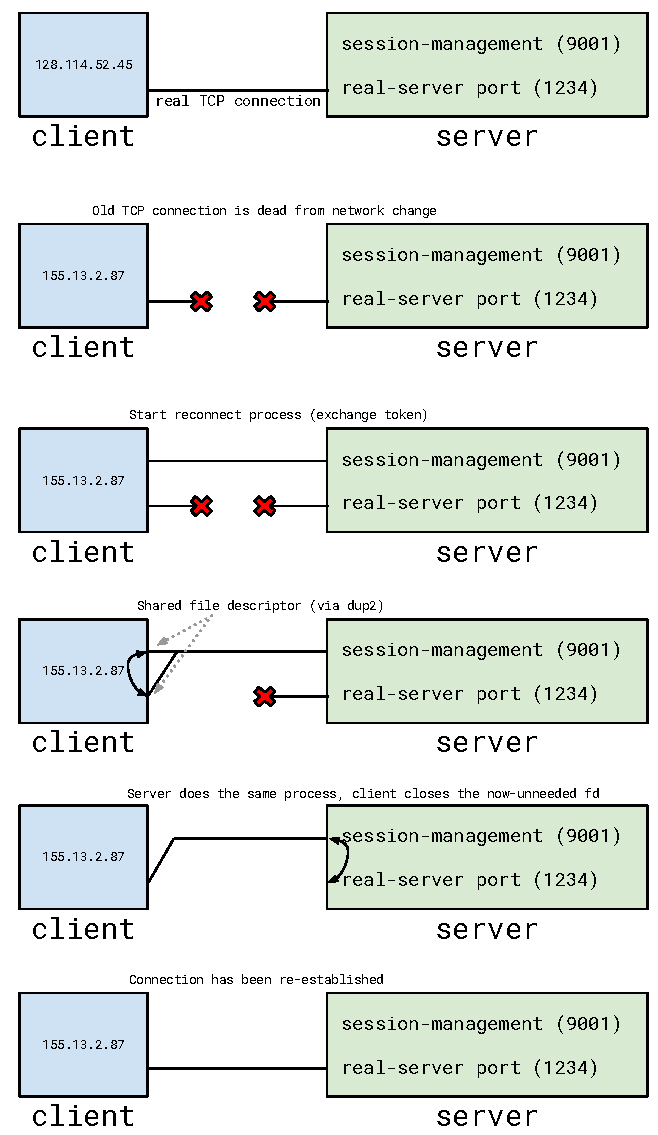
\includegraphics[width=80mm,height=127mm]{fig/reconn_diag}
	\caption{The reconnection process. The client moves networks, causing its
	address to change, which breaks the TCP connection. The client and server
	negotiate a new connection via the session management port, which is then
	used to replace the old connection file descriptors, allowing transparent
	reconnection. The two lines of text in the server's box represents logically
	what a given file descriptor is used for in the server; obviously there is
	no direct connection between ports and file descriptors and the diagram
	should not be interpreted to mean that there is.}
	\label{fig:recproc}
\end{figure}

Upon receiving the signal, the client opens a new connection to the session
management port. It sends a \texttt{SESSION RECONNECT} packet, and waits for an
acknowledgement from the server. If acknowledged, it sends the server the
session token, followed by replacing the file descriptor that referred to the
now-dead TCP connection that is being reestablished. Meanwhile, upon receiving
the session token, the server does a similar operation to replace its end of the
now-dead TCP connection with a new one. The new connection that they replace the
old one with is the TCP connection that was established via the session
management port. The effect is that the server and client have a new,
functioning TCP connection between them without them noticing that it replaced a
dead one. Interaction can now continue unimpeded.

\section{Implementation Details}
\label{sec:impl}

The design is somewhat straight forward, with the basic idea being to replace an
old, dead TCP connection with a new one by manipulating file descriptors.
However, there are a number of design details that are worth discussing.

\paragraph{Replacing File Descriptors}
The core functionality of reconnection is done by replacing the file descriptor
that refers to the old TCP connection with one that refers to a new connection.
This can be accomplished by the \texttt{dup2} systemcall, which duplicates a
given file descriptor into another provided file descriptor, closing the target
if it is open. This is exactly what we want, however there are some details.
Firstly, this code must run in isolation. For the client, this is simple---we
are already triggering reconnection by signal handling, so while we are handling
the signal to interact with the session-server, we can also use \texttt{dup2} to
replace our end of the dead TCP connection once the session token has been
exchanged. Since we are running in a signal handler, no other code can execute
(assuming single-threaded clients). Once our signal handler completes, the file
descriptor will be replaced and the client can continue normally.

However, if the application was executing inside a system call, the default
action is to return from the system call with \texttt{EINTR} (interrupted system
call). This may be unexpected for applications, so we specify the
\texttt{SA\_RESTART} flag for the signal handler to that system calls are
restarted instead. An added benefit of restarting system calls is that system
calls that were started with the old, dead TCP connection will use the new TCP
connection. This is because the file descriptor \textit{number} has not changed,
only the underlying file description object in the kernel.


\paragraph{Server Session Support}
The server is quite a bit more complicated for two reasons: it does not have a
convenient linearizable operation that signals it that a reconnect is happening,
and it must listen on multiple ports. The real server listens on its normal port
for new TCP connections, but the session-server must also accept new connections
on the session management port. To facilitate this, the session-server starts a
background thread that listens on that port. When it receives a \texttt{SESSION
RECONNECT} packet and successfully exchanges a session token, it stops the real
server's main thread before replacing the file descriptor for the old connection
with the new one in the same was as described above (with \texttt{dup2}).
Finally, it resumes the real server's main thread.

Stopping a restarting the main thread is done by having it register two signal
handlers during initialization, \texttt{SIGUSR1} and \texttt{SIGUSR2}. When the
server receives \texttt{SIGUSR1}, its handler masks all signals except
\texttt{SIGUSR2} and calls \texttt{sigsuspend}, allowing it to wait to be woken
back up. The session management thread then does its work before signaling the
main thread with \texttt{SIGUSR2}. The signal handlers are specified to be
\texttt{SA\_RESTART}, for the same reason described above.

A final detail for both the client and the server is that they should mask all
signals (except \texttt{SIGUSR2}) in the case of the server so that while they
are executing critical code (replacing file descriptors), they do not get
interrupted. Additionally, the masks will allow the signals to be delivered
normally after the reconnection operation, in case the application needs a
particular signal. The session-server gets this functionality easily by masking
all signals in the session management thread, forcing all signals to be
delivered to the main thread, which only masks signals while it is suspended.
Additionally, the signals that are used by the session code may be used
by the applications as well. However, the session code must not allow the
application to override its signal handlers, lest it break its functionality.
Thus, the session code overrides the \texttt{sigaction} library call as well and
records attempts to register new signal handlers by the application. Then, when
a signal is delivered, the session code can execute the code it needs to execute
before finally delivering the signal to the application.

\section{Microbenchmarks}

The two primary operations supported by \sesh are session establishment and
session reconnection. Each operation is initiated by the client and has a
portion completed by the client that is synchronous with the algorithm used by
the server. That is, the client initiates an operation, does some work, notifies
the server, and waits for an \texttt{ack} message. As such, we expect the client
operations to take strictly longer than the server operations. This is
beneficial, since we prefer to make the clients wait longer than the server
because servers are often multiplexed and cannot tolerate longer interruptions
of service.

Experiments were done on a Linux machine using the loopback network
interface on an Intel Ivybridge i5 processor. To measure the results, I used
\texttt{LD\_PRELOAD} to inject the libraries into \texttt{netcat} before
instructing it to reconnect 2000 times. The process of establishing a connection
was scripted, and also run 2000 times. Results were analyzed using the Pilot
statistical analysis program~\cite{pilot}, and the error bars in the graphs
represent 95\% confidence intervals.

\begin{figure}[!htb]
	\centering
	\includegraphics[width=70mm]{fig/time_est}
	\caption{Latency for establishing a TCP connection using \sesh. The time
	represents the additional overhead of the session functionality over that of
	a normal TCP connection establishment.}
	\label{fig:est}
\end{figure}

Figure~\ref{fig:est} shows the latency for session establishment. The extra
variability in the client's latency is explained by the synchronous nature of
the protocol---the client's latency is influenced by network latency. The
server, on the other hand, performs only a small number of operations to
allocate and record the session, and generate a random token (the prototype uses
the built-in C library random functions). The client must also record the token,
and it must create and establish a TCP connection to the session management
port, whereas the server is already listening and so has less overhead in
setting up the extra socket.
The latency of establishment is well within network latency magnitudes, making
it a tolerable overhead (especially since it is an uncommon operation).

\begin{figure}[!htb]
	\centering
	\includegraphics[width=70mm]{fig/time_recon}
	\caption{Latency for reconnecting with a new TCP connection between a client
	and a server with a previously established session.}
	\label{fig:recon}
\end{figure}

Figure~\ref{fig:recon} describes the reconnection latency. Again, the client's
latency is influenced by network latency for the same reasons, and is similar to
the session establishment latency for all the reasons listed above. However, the
server has a significant amount of additional work it must do, some of which is
asynchronous with the client. This means that it takes much longer to reconnect
than to establish, but it does not affect the client's latency as much. The
numbers are still within normal network latency for the use-cases we expect for
\sesh, meaning the delays are tolerable. Finally, the server's latency is more
variable since it involves two threads signaling each other.


\section{Related Work}

Providing ``mobile IP'' services is common in cell networks, since users are
largely truly mobile and so need a built-in method to have changing IP addresses
are part of the network design~\cite{ltemob,mobileip,Kurose}. While this largely
solves the problem for cell networks, it does not provide interoperability for
cell-phones that reconnect to WiFi networks, which do not have the same
functionality. This limitation is indicative of a larger limitation---the
network must support the requirements of a mobile-IP infrastructure. This
contrary to arguments in~\cite{Saltzer}, because it requires support through the
whole stack. Furthermore, these solutions often require support by client
applications and potentially servers (which may or may not understand the
complexities of mobile-IP services, resulting in errant behavior).
OpenFlow~\cite{McKeown} also
provides features for mobility with flows, but also requires extensive support
in the hardware and network.

Other projects and papers, such as Chandrashekar's Service Oriented
Internet~\cite{chandrashekar2003service} and Saif's Service-Oriented Network
Sockets~\cite{Saif} discuss designs for, essentially, session layer network designs.
While \sesh would eventually provide more session-like features than
simple reconnect and session tokens, that work is outside the scope of a class
project. However, much of the work in the aforementioned papers is extremely
relevant to the future of a library such as \sesh.

A session layer protocol that explicitly provides reconnection is
\textit{fived}~\cite{wasptr-15-01}. \textit{Fived} runs as a daemon on both
endpoints, through which clients and servers can establish sessions.
\textit{Fived} provides a number of services that \sesh does not yet,
but should in the future, support, such as service enumeration. However,
\textit{fived} incurs additional overhead by running as a daemon, whereas
\sesh runs as libraries that interpose library calls, improving
performance.

Numerous projects focus on problem-avoidance for reconnecting dead TCP
connections~\cite{mosh,autossh,screen,tmux}. Solutions range from implementing
sessions on the server (which require forethought and explicit use of tools), to
reparenting processes to continue running on hangup (which is not a session), to
reestablishing a new connection automatically (which is also not a session). All
these solutions lack the usability and transparency of true sessions.

\section{Future Work}

\Sesh focused only on providing a reconnection service for dead TCP connections
after network movement. However, it could be drastically extended to provide
more features of a session layer. For example, a \sesh daemon could run on each
machine in order to manage shared resources between all applications that use
the \sesh library to combine all session management for different applications
on a given machine into one process. Of course, the \sesh library would still be
used to reconnect TCP connections and perform the actual establishment in order
to not lose the performance of shared libraries over a daemon, but the presence
of a daemon would allow multiple \sesh-enabled servers on one machine (which is
currently not possible). It would also help support network changes while data
is being sent, which could currently result in some data loss. Data is sent both
across the network and also to the session server, which can keep its own TCP
buffer in order to replay stored data into the new connection after a
reconnection attempt. If applications are written to be aware of a \sesh daemon,
it can provide services similar to that of \textit{fived}~\cite{wasptr-15-01},
such as service discovery and multiplexing,
while also providing improved performance and transparent support for legacy
applications.

While \sesh works at decoupling client identity from the client's address, it
does not do the same for the server. An interesting future work could be to
extend the above daemon idea with the ability to save a session (including token
and temporary buffers) and move it to another machine, following a
``forwarding'' response when the client tries to use the old server address.

A severe limitation of \sesh in its current form is support for \texttt{fork}ing
servers. For example, \texttt{ssh} cannot be imbued with session support right
now because its management of file descriptors and processes is much more
complex and it is out of the scope of a class project to support this. However,
it is not outside the realm of possibility; the \sesh library would need to
interpose on \texttt{fork} and \texttt{exec} to inject itself into a child's
address space and continue to function there.

Finally, the security of \sesh could stand to be improved. Currently, only the
token is necessary to reestablish a connection. Future sessions could be
protected by a login primitive which would only allow a session to reconnect
after user identity is confirmed. Another problem is that the token is exchanged
in the clear, meaning that man-in-the-middle attacks are possible to hijack
sessions. All of these security problems are outside the scope of the class,
considering the difficulty in engineering the basic proof-of-concept itself. A
solution would be two-fold: use session-based encryption negotiated via either
public/private key encryption (like ssh) or password-based tokens (like
Kerberos). In any case, to perform the reconnection, the client and server
should use challenge/response authentication to avoid sending the session token
in the clear.

\section{Conclusion}

Networking technologies will never stop evolving, and will never stop
encountering problems that need to be solved. Often these problems manifest as
minor inconveniences for end users, but their solutions can often have
significant impact for networking services and design in the future. Providing
support for reconnections for TCP could make many services much more reliable,
providing support for decoupled identity from addresses could allow much easier
mobility of users across machines, and providing a unified method for
establishing secure connections could change networking security drastically for
the better.

But it does not have to stop there; improving the mobility of
endpoints in a communication could improve the way that data and services move
about in large, complicated networking environments and data centers. If a
service on a machine can easily move to another through the use of sessions, we
could flip load-balancing on its head. The service is automatically moved from
higher-performance servers to lower-performance but more power-efficient servers
when its load decreases, and can be automatically moved back when load
increases. This is made much easier with sessions, because existing connections
are trivially moved. Another implication is that of ``long-paused'' connections;
that is, connections between two machines were one (or both) may sleep or
power-down. When they resume, they may wish to resume what they were doing,
including communicating with the other machine. An example could be a sensing
device (or an IoT device) that powers down for a large amount of time, storing
session data in non-volatile memory, and then powers back on, resuming the
session.

No matter how its used, the idea is interesting. Greater support for network
mobility in an environment that did not account for such a feature is
interesting has has merit for future discussion and exploration.










\bibliography{sesh}
\bibliographystyle{plainnat}

\end{document}

